\documentclass{standalone}
\usepackage{tikz}
\usetikzlibrary{automata,positioning,arrows,shapes,decorations,calc,
arrows.meta,fit}
\usetikzlibrary{decorations.pathmorphing}
\usetikzlibrary{decorations.pathreplacing}
\usetikzlibrary{decorations.shapes}
\usetikzlibrary{decorations.text}
\usetikzlibrary{decorations.markings}
\usetikzlibrary{decorations.fractals}
\usetikzlibrary{decorations.footprints}

\tikzset{
roundnode/.style={rectangle, draw=black, very thick, text width=20mm, minimum height=1cm},
phasenode/.style={rectangle, draw=black, very thick, text width=3cm, minimum height=1cm},
phasenodeBis/.style={rectangle, draw=black, very thick, minimum width=9cm, minimum height=5cm},
>={Latex[width=2mm,length=2mm]},
base/.style = {rectangle, rounded corners, draw=black,
                         minimum width=4cm, minimum height=1cm,
                         text centered, font=\sffamily},
%every picture/.style={/utils/exec={\sffamily}}
every edge quotes/.append style={font=\scriptsize, align=center, auto}% style for edge labels
}

\begin{document}
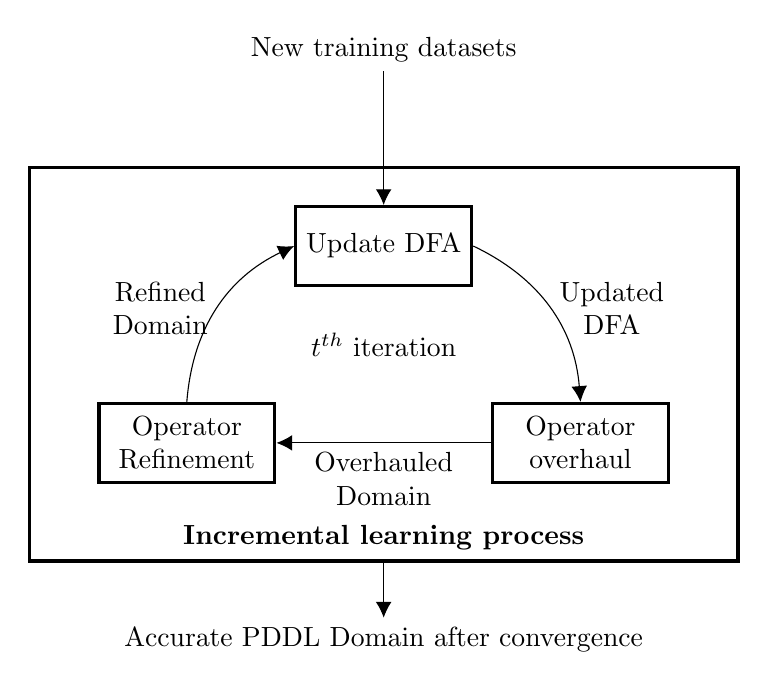
\begin{tikzpicture}[node distance=1.5cm, align=center]

%Automaton nodes
\node[phasenodeBis] (phase2Bis) at(0,-1.5)  {};
\node[roundnode] (grammar) at(0,0)  {Update DFA};
\node[roundnode] (overhaul) at(2.5,-2.5)  {Operator overhaul};
\node[roundnode] (refinement) at(-2.5,-2.5)  {Operator Refinement};

\node[text width=4cm] (batch) at(0,2.5)  {New training datasets};
\node (iteration) at(0,-1.25)  {$t^{th}$ iteration};

\draw[->] (batch.south) --node[left] {} (grammar.north) ;
% \draw[->] (initial.south) --node[right] {} (phase.north) ;
% \draw[->] (phase.south) --node[right] {Initial Domain $\delta^0$} (grammar.north east) ;
\path[->] (grammar.east) edge[bend left] node[right] {Updated\\ DFA} (overhaul.north) ;
\draw[->] (overhaul.west) --node[below] {Overhauled\\ Domain} (refinement.east) ;
\path[->] (refinement.north) edge[bend left] node[left] {Refined\\ Domain} (grammar.west) ;

% \draw [decorate,decoration={brace,amplitude=10pt,mirror,raise=6pt},yshift=0pt] (-4,-3.15) -- (4,-3.15);

\node (phase2) at(0, -3.7) {\textbf{Incremental learning process}};
\node (output) at(0, -5) {Accurate PDDL Domain after convergence};

\draw[->] (phase2Bis.south) -- (output.north) ;
\end{tikzpicture}
\end{document}
